\documentclass[15pt]{beamer}
\usepackage{tikz}
\usepackage{graphicx}
\usepackage{booktabs}
\usetikzlibrary{positioning, arrows.meta}

\usetheme{Berkeley}
\usecolortheme{default}

\title[Subprime Housing]
{Long Tail Impacts of Early 2000s Subprime Loans On Today's Housing Market}
\author[Matthew, Robson]
{M. ~Robson\inst{1}}

\institute[ICR]
{
  \inst{1}%
  Austin Branch\\
  Institute of Computing in Research
}

\date[July 2026]
{July 2026}


\logo{\begin{tikzpicture}
        \hspace{-0.78cm}
        \raisebox{-0.73cm}{
\includegraphics[width=0.12\textwidth]{logo.jpeg}}
\end{tikzpicture}}

%% finally
\begin{document}

\frame{\titlepage}

%%%%%%%%%%%%%%%%%%%%%%%%%%%%%%%%%%%%%%%%%%%%%%%%%%%%%%%%%%%%%%%%%%

\begin{frame}
\frametitle{What is a Subprime Loan?}

\begin{block}{subprime (adjective)} %% https://en.wikipedia.org/wiki/Subprime_lending
    Subprime loans are characterized by higher interest rates, poor quality collateral, and less favorable terms in order to compensate for higher credit risk.
\end{block}

\begin{itemize}
    \item Subprime loans are generally given to people with a FICO score of less than 670.  
    \item Subprime loans usually have a rate spread of greater than 3\%.
\end{itemize}


\end{frame}

\begin{frame}{MBS and CDOs} %%% https://en.wikipedia.org/wiki/File:CDO_-_FCIC_and_IMF_Diagram.png
    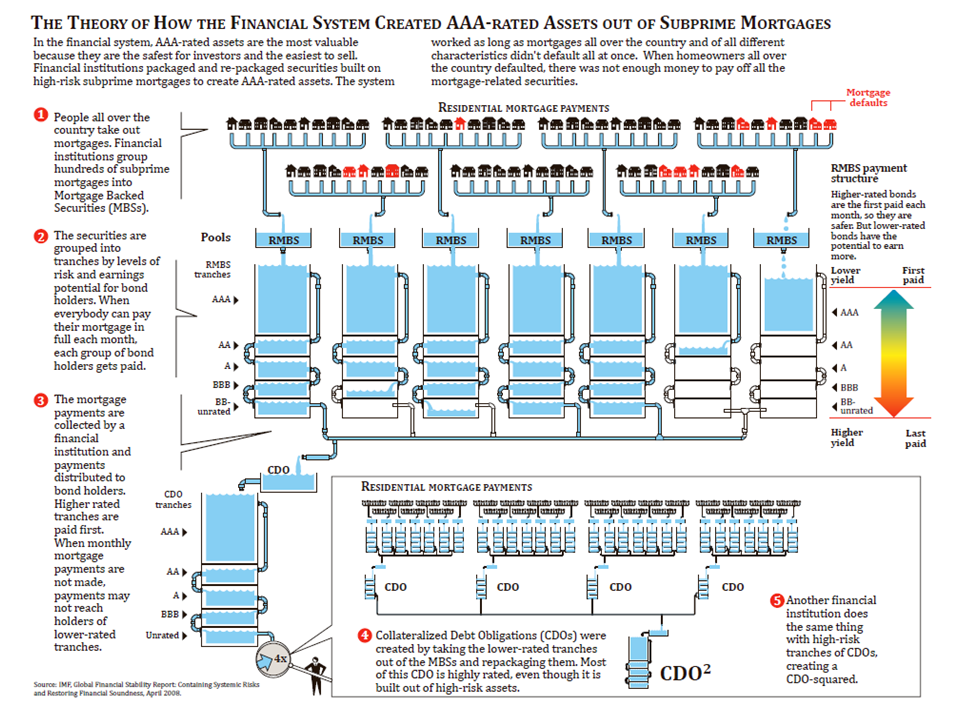
\includegraphics[width=\textwidth]{CDO_-_FCIC_and_IMF_Diagram.png}
\end{frame}

%%%%%%%%%%%%%%%%%%%%%%%%%%%%%%%%%%%%%%%%%%%%%%%%%%%%%%%%%%%%%%%%%%

\begin{frame}
\frametitle{The 2008 Financial Crisis}

\begin{columns}
    \column{0.5\textwidth} %% https://en.wikipedia.org/wiki/2008_financial_crisis

    \begin{itemize}
        \item Causes:
        \begin{itemize}
            \item Defaults on Subprime Loans
            \item Over-leveraging
            \item Poor Rating Standards
        \end{itemize}
        \item Consequences
        \begin{itemize}
            \item Massive Financial Downturn
            \item People lost their houses
            \item Banks went bankrupt
        \end{itemize}
    \end{itemize}
    
    \column{\textwidth}
    %% David Shankbone, CC BY-SA 3.0 <http://creativecommons.org/licenses/by-sa/3.0/>, via Wikimedia Commons
    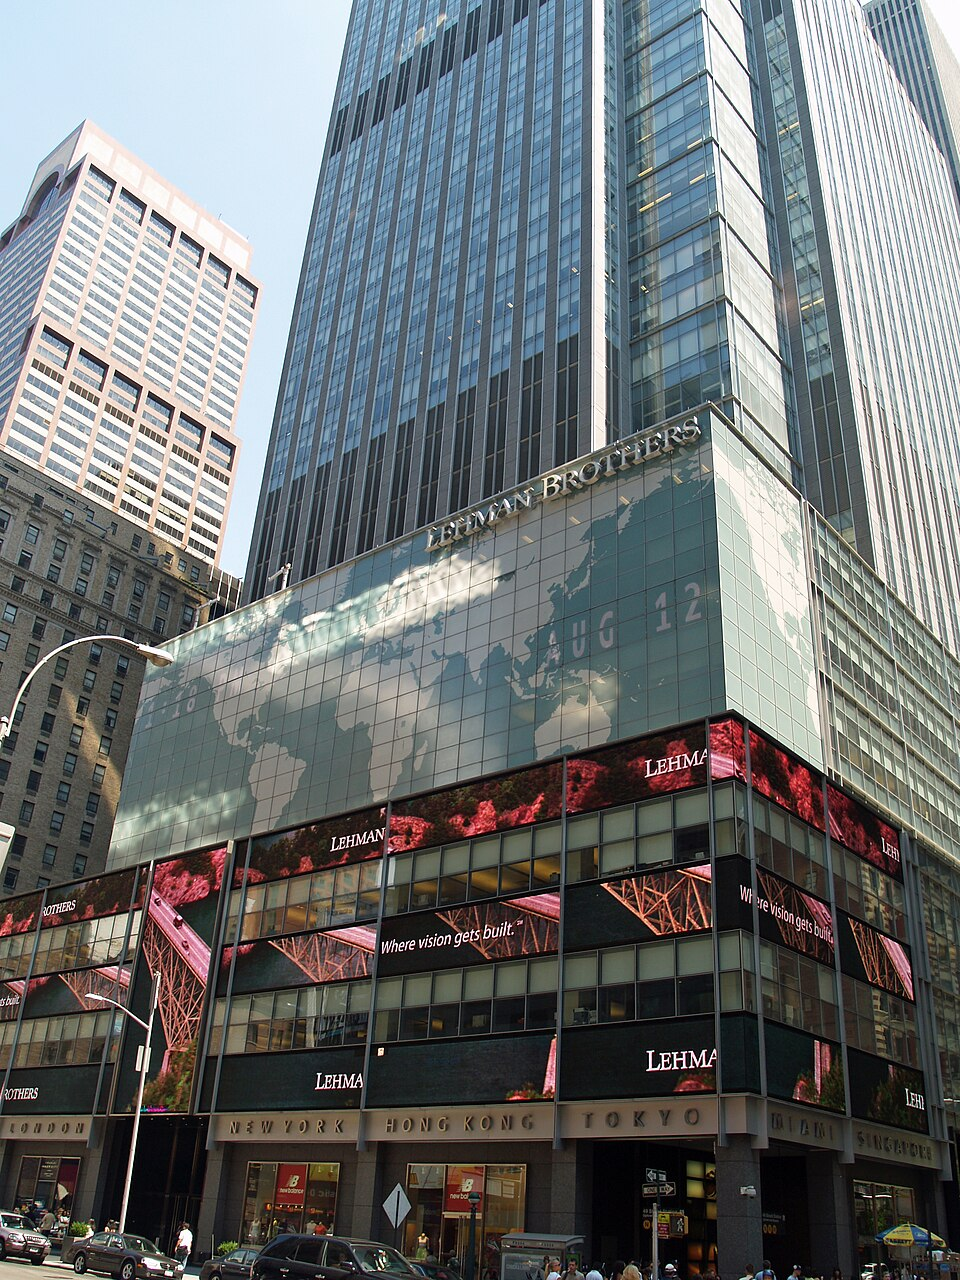
\includegraphics[width=0.5\textwidth]{960px-Lehman_Brothers_Times_Square_by_David_Shankbone.jpg}
\end{columns}


\end{frame}

%%%%%%%%%%%%%%%%%%%%%%%%%%%%%%%%%%%%%%%%%%%%%%%%%%%%%%%%%%%%%%%%%%

\begin{frame}{Framing the Study}
  \centering
  \vspace{0.1cm}
  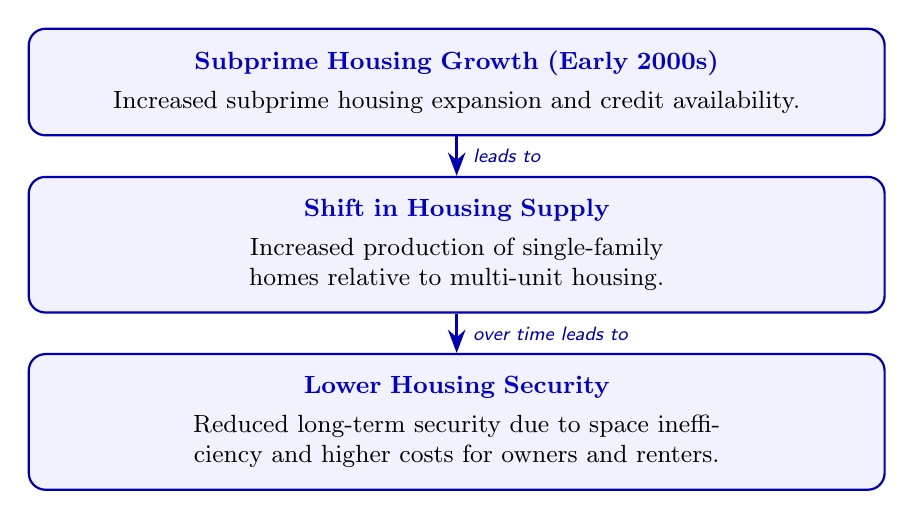
\begin{tikzpicture}[
    node distance=0.5cm,
    causal block/.style={
      rectangle,
      draw=blue!70!black,
      fill=blue!5,
      thick,
      rounded corners=6pt,
      align=center,
      text width=0.85\linewidth,
      inner sep=8pt,
      font=\small
    },
    causal arrow/.style={
      -Stealth,
      very thick,
      color=blue!70!black
    }
  ]

    \node[causal block] (block1) {
      \textbf{\color{blue!80!black}Subprime Housing Growth (Early 2000s)}\\[3pt]
      Increased subprime housing expansion and credit availability.
    };

    \node[causal block, below=of block1] (block2) {
      \textbf{\color{blue!80!black}Shift in Housing Supply}\\[3pt]
      Increased production of single-family homes relative to multi-unit housing.
    };

    \node[causal block, below=of block2] (block3) {
      \textbf{\color{blue!80!black}Lower Housing Security}\\[3pt]
      Reduced long-term security due to space inefficiency and higher costs for owners and renters.
    };

    \draw[causal arrow] (block1) -- (block2) 
      node[midway, right=2pt, font=\scriptsize\sffamily, color=blue!70!black] {\textit{leads to}};
      
    \draw[causal arrow] (block2) -- (block3) 
      node[midway, right=2pt, font=\scriptsize\sffamily, color=blue!70!black] {\textit{over time leads to}};

  \end{tikzpicture}
\end{frame}

%%%%%%%%%%%%%%%%%%%%%%%%%%%%%%%%%%%%%%%%%%%%%%%%%%%%%%%%%%%%%%%%%%

\begin{frame}
\frametitle{Why do we care?}

\begin{columns}
    \column{0.5\textwidth} %% https://en.wikipedia.org/wiki/2008_financial_crisis

    \begin{itemize}
        \item Homelessness is increasing
        \item Overcrowding in homes
        \item Crime rate 
        \item Poor Housing Quality
        \item Cost Burden is Increasing %% look for inforaphic
    \end{itemize}
    
    \column{\textwidth}
    %% https://endhomelessness.org/state-of-homelessness/
    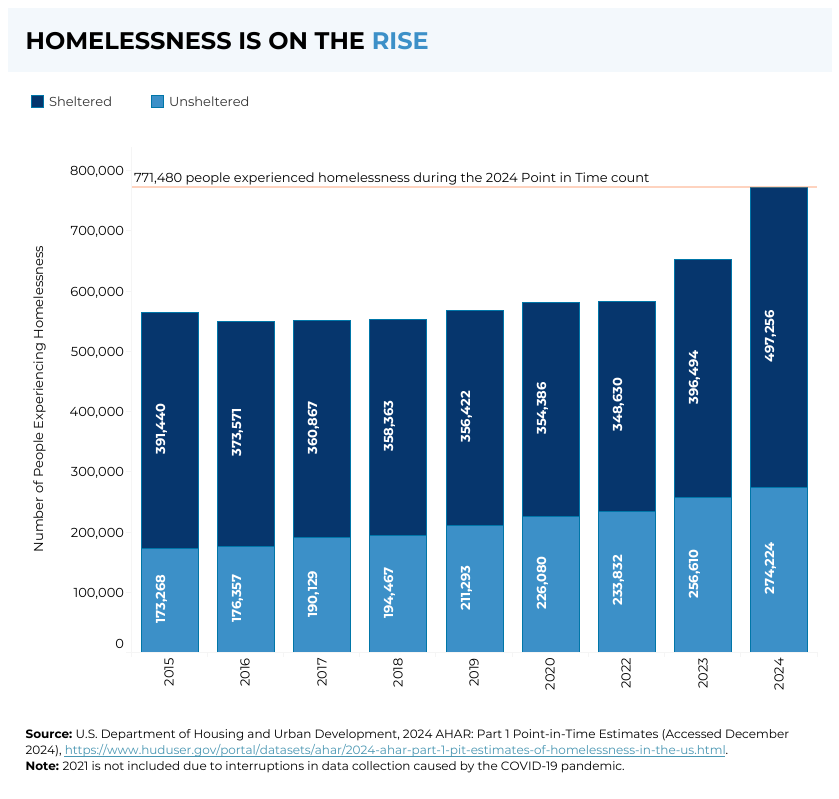
\includegraphics[width=0.5\textwidth]{PIT Trend.png}
\end{columns}

\end{frame}

%%%%%%%%%%%%%%%%%%%%%%%%%%%%%%%%%%%%%%%%%%%%%%%%%%%%%%%%%%%%%%%%%%

\begin{frame}
\frametitle{Data Collection}

\begin{block}{Sources}
    \begin{itemize}
        \item ACS --- I used the American Community Survey (5yr) for the demographic and economic data for each tract. Additionally, this was the source for the measures of housing insecurity. 
        \item HMDA --- The Home Mortgage Disclosure Act passed allows anyone to download a list of every housing loan taken out every year, including information such as loan amount, rate spread, HOEPA status, etc.
    \end{itemize}

    
\end{block}

\begin{block}{Packages}
    \begin{itemize}
        \item Polars / Pandas / GeoPandas
        \item Statsmodel / Bambi / Seaborn
    \end{itemize}
\end{block}

\end{frame}

%%%%%%%%%%%%%%%%%%%%%%%%%%%%%%%%%%%%%%%%%%%%%%%%%%%%%%%%%%%%%%%%%%

\begin{frame}
\frametitle{Important Variables}

\begin{block}{Dependent Variables}
    Housing Insecurity
    \begin{itemize}
        \item Cost Burden
        \item Overcrowding
    \end{itemize}
\end{block}

\begin{block}{Independent Variable}
    \begin{itemize}
        \item Subprime Rate
    \end{itemize}
\end{block}

\begin{block}{Controlling Variables}
    \begin{itemize}
        \item Demographic: Race, Undergraduate Percentage
        \item Economic: Income, Unemployment, Poverty Rate
    \end{itemize}
\end{block}


\end{frame}

%%%%%%%%%%%%%%%%%%%%%%%%%%%%%%%%%%%%%%%%%%%%%%%%%%%%%%%%%%%%%%%%%%

\begin{frame}
\frametitle{Results --- Overcrowding Rate}

\centering
\setlength{\tabcolsep}{2.5pt}
\renewcommand{\arraystretch}{0.72}
\resizebox{\linewidth}{!}{%
{\scriptsize
\begin{tabular}{l c c c c}
\toprule
 & Baseline & (2) & (3) & (4) \\
\midrule
Unemployment\_PCT         &             & -0.0002**  &            & -0.0008*** \\
                          &             & (0.0001)   &            & (0.0001)   \\
Poverty\_Rate\_PCT        &             & 0.0009***  &            & 0.0002***  \\
                          &             & (0.0000)   &            & (0.0000)   \\
Median\_Household\_Income &             & 0.0001***  &            & 0.0001***  \\
                          &             & (0.0000)   &            & (0.0000)   \\
White\_pct                &             &            & -0.0013*** & -0.0013*** \\
                          &             &            & (0.0000)   & (0.0000)   \\
Black\_pct                &             &            & -0.0012*** & -0.0011*** \\
                          &             &            & (0.0000)   & (0.0000)   \\
Hispanic\_pct             &             &            & -0.0002*** & -0.0002*** \\
                          &             &            & (0.0000)   & (0.0000)   \\
Undergrad\_pct            &             &            & -0.0004*** & -0.0005*** \\
                          &             &            & (0.0000)   & (0.0000)   \\
Subprime\_pct             & 0.1562***   & 0.1029***  & 0.0062     & 0.0024     \\
                          & (0.0048)    & (0.0065)   & (0.0074)   & (0.0073)   \\
Intercept                 & 0.0138***   & 0.0039***  & 0.1438***  & 0.1425***  \\
                          & (0.0005)    & (0.0012)   & (0.0028)   & (0.0030)   \\
\midrule
R-squared                 & 0.0270      & 0.0581     & 0.3968     & 0.4044     \\
Adj. R-squared            & 0.0270      & 0.0580     & 0.3967     & 0.4043     \\
N                         & 44,611      & 44,489     & 44,611     & 44,489     \\
\bottomrule
\multicolumn{5}{l}{\tiny Standard errors in parentheses. * $p<0.1$, ** $p<0.05$, *** $p<0.01$} \\
\multicolumn{5}{l}{\tiny (2) Baseline + Economic, (3) Baseline + Demographic, (4) All Variables}
\end{tabular}
}
}

\end{frame}

%%%%%%%%%%%%%%%%%%%%%%%%%%%%%%%%%%%%%%%%%%%%%%%%%%%%%%%%%%%%%%%%%%

\begin{frame}
\frametitle{Results --- Cost Burden}

\centering
\setlength{\tabcolsep}{2.5pt}
\renewcommand{\arraystretch}{0.72}
\resizebox{\linewidth}{!}{%
{\scriptsize
\begin{tabular}{l c c c c}
\toprule
 & Baseline & (2) & (3) & (4) \\
\midrule
Unemployment\_PCT         &             & 0.2010***   &            & -0.0043    \\
                          &             & (0.0158)    &            & (0.0156)   \\
Poverty\_Rate\_PCT        &             & -0.0059     &            & -0.2112*** \\
                          &             & (0.0075)    &            & (0.0082)   \\
Median\_Household\_Income &             & 0.0786***   &            & 0.0266***  \\
                          &             & (0.0021)    &            & (0.0022)   \\
White\_pct                &             &             & -0.2518*** & -0.2754*** \\
                          &             &             & (0.0065)   & (0.0056)   \\
Black\_pct                &             &             & -0.1558*** & -0.1247*** \\
                          &             &             & (0.0071)   & (0.0064)   \\
Hispanic\_pct             &             &             & -0.0795*** & -0.0678*** \\
                          &             &             & (0.0078)   & (0.0067)   \\
Undergrad\_pct            &             &             & 0.1269***  & 0.0525***  \\
                          &             &             & (0.0036)   & (0.0039)   \\
Subprime\_pct             & -36.8989*** & -12.3028*** & -19.8165***& -25.1691***\\
                          & (1.0786)    & (1.4482)    & (1.7683)   & (1.6327)   \\
Intercept                 & 20.2390***  & 10.9132***  & 32.2269*** & 37.7072*** \\
                          & (0.1329)    & (0.3008)    & (0.7134)   & (0.6408)   \\
\midrule
R-squared                 & 0.0291      & 0.0722      & 0.2389     & 0.2981     \\
Adj. R-squared            & 0.0291      & 0.0721      & 0.2389     & 0.2980     \\
N                         & 44,716      & 44,489      & 44,716     & 44,489     \\
\bottomrule
\multicolumn{5}{l}{\tiny Standard errors in parentheses. * $p<0.1$, ** $p<0.05$, *** $p<0.01$} \\
\multicolumn{5}{l}{\tiny (2) Baseline + Economic, (3) Baseline + Demographic, (4) All Variables}
\end{tabular}
}
}

\end{frame}
%%%%%%%%%%%%%%%%%%%%%%%%%%%%%%%%%%%%%%%%%%%%%%%%%%%%%%%%%%%%%%%%%%

\begin{frame}{Results --- Nationwide Subprime Housing}
  \centering
  % \vspace*{-0.3cm}
  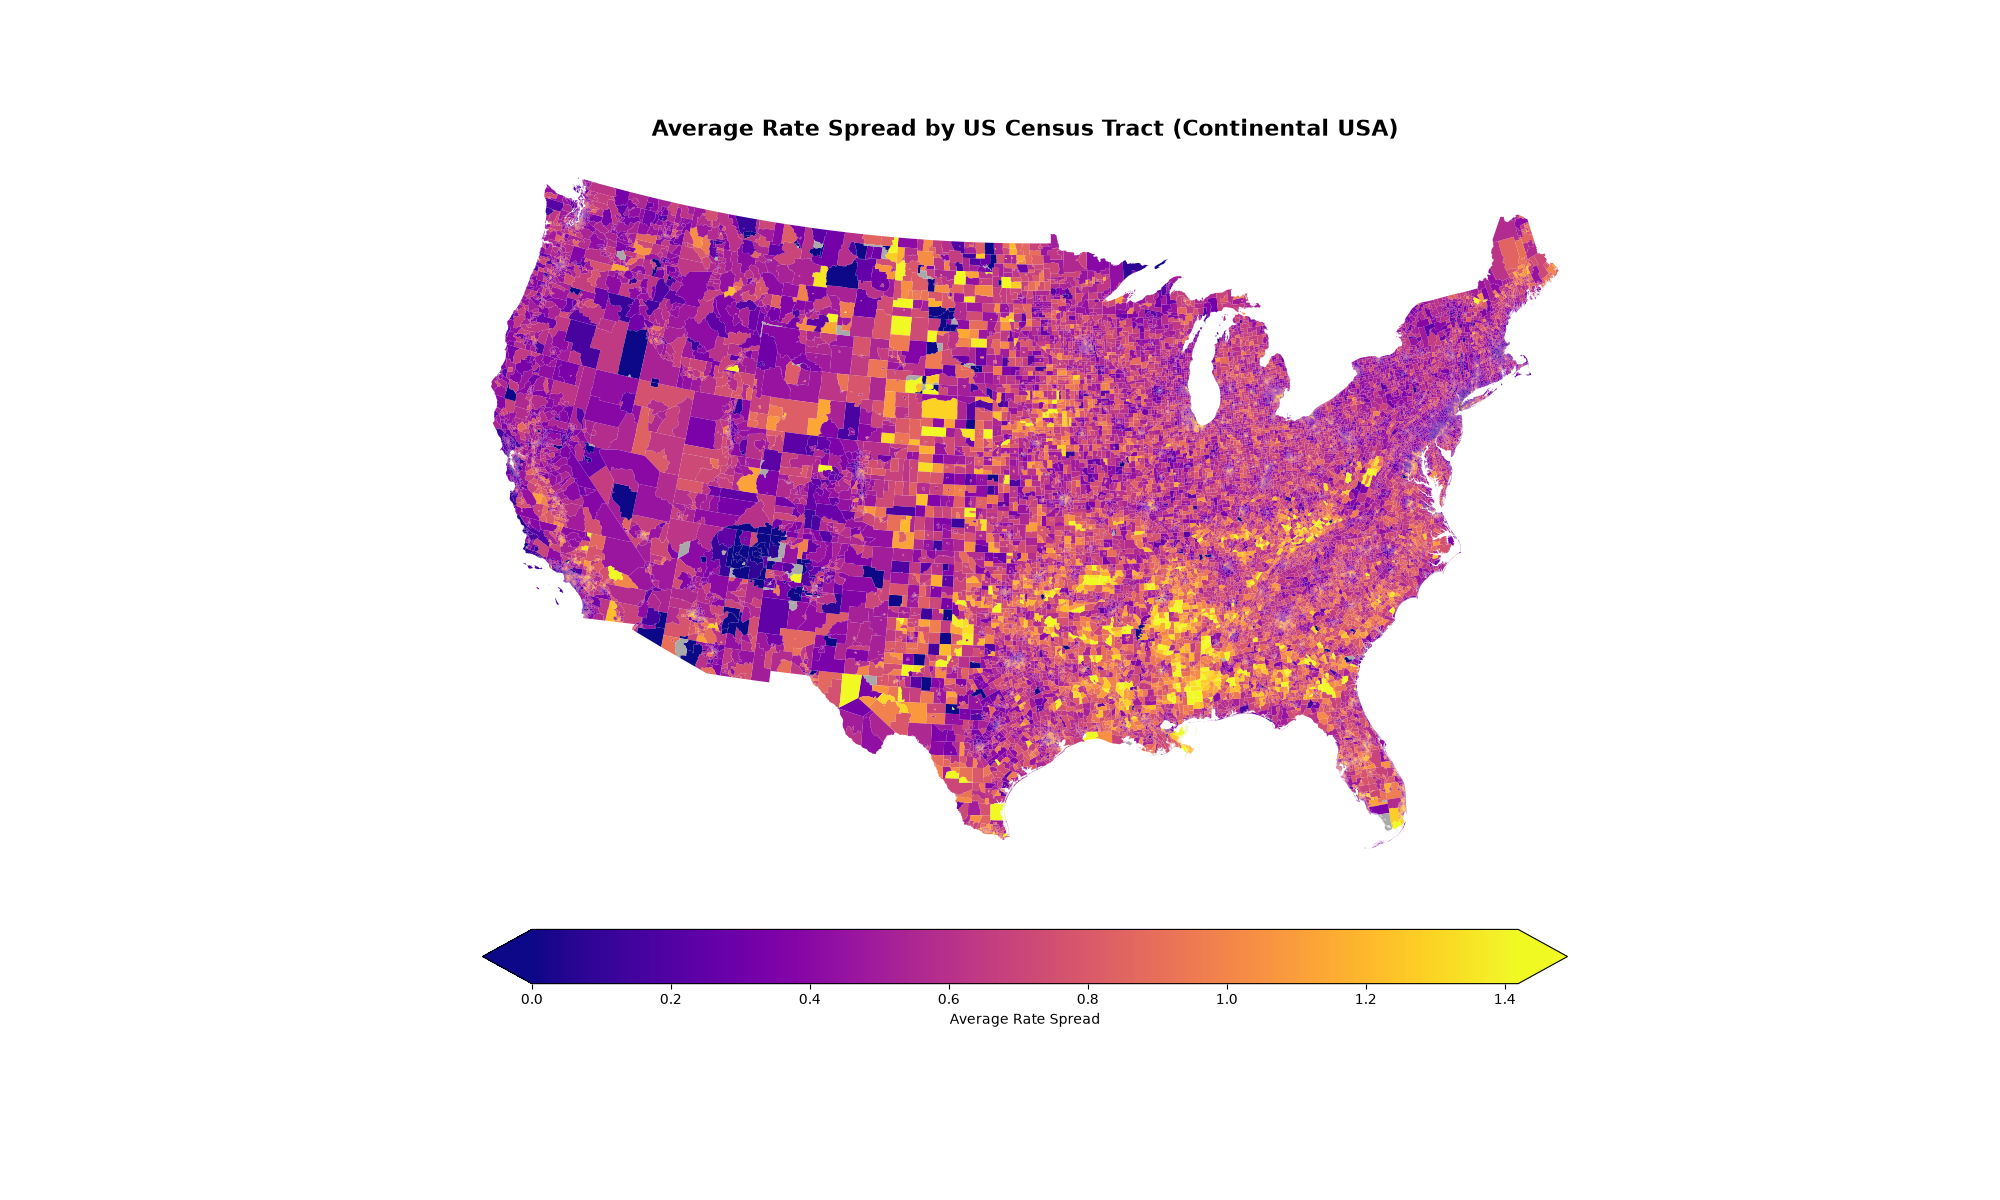
\includegraphics[height=\textheight, keepaspectratio,trim={11cm, 2cm, 11cm, 2cm}, clip]{SubprimeLoanSpread2006.png}
\end{frame}

%%%%%%%%%%%%%%%%%%%%%%%%%%%%%%%%%%%%%%%%%%%%%%%%%%%%%%%%%%%%%%%%%%

\begin{frame}
\frametitle{Discussion}

\begin{block}{Key Findings}
    \begin{itemize}
        \item \textbf{Overcrowding \& Demographics:} The relationship between subprime lending and overcrowding becomes statistically insignificant once demographic controls are added
        \item \textbf{Housing Cost Burden:} Higher historical subprime rates strongly correlate with lower current cost burdens across all models
    \end{itemize}
\end{block}

\begin{block}{Implications}
    Post-crisis price adjustments may have led to the negative association between subprime rates the cost burden. Future work could include attempt to normalize for economic status at the time of the loan creation.
\end{block}

\end{frame}

\begin{frame}{Conclusion}

\begin{block}{Other Bubbles}
    \begin{itemize}
        \item AI Bubble
        \begin{itemize}
            \item Data Center Production
            \item Environmental Impacts
        \end{itemize}
        \item Dotcom Bubble
        \begin{itemize}
            \item Internet Infrastructure
            \item Venture Capital
        \end{itemize}
    \end{itemize}
\end{block}

AI expansion is driving data center construction which could have longer term benefits to people in the future like that of the long term benefits of internet construction.

\end{frame}

\end{document}
